\documentclass[letterpaper,12pt,oneside]{article}\usepackage[]{graphicx}\usepackage[]{color}
%% maxwidth is the original width if it is less than linewidth
%% otherwise use linewidth (to make sure the graphics do not exceed the margin)
\makeatletter
\def\maxwidth{ %
  \ifdim\Gin@nat@width>\linewidth
    \linewidth
  \else
    \Gin@nat@width
  \fi
}
\makeatother

\definecolor{fgcolor}{rgb}{0.345, 0.345, 0.345}
\newcommand{\hlnum}[1]{\textcolor[rgb]{0.686,0.059,0.569}{#1}}%
\newcommand{\hlstr}[1]{\textcolor[rgb]{0.192,0.494,0.8}{#1}}%
\newcommand{\hlcom}[1]{\textcolor[rgb]{0.678,0.584,0.686}{\textit{#1}}}%
\newcommand{\hlopt}[1]{\textcolor[rgb]{0,0,0}{#1}}%
\newcommand{\hlstd}[1]{\textcolor[rgb]{0.345,0.345,0.345}{#1}}%
\newcommand{\hlkwa}[1]{\textcolor[rgb]{0.161,0.373,0.58}{\textbf{#1}}}%
\newcommand{\hlkwb}[1]{\textcolor[rgb]{0.69,0.353,0.396}{#1}}%
\newcommand{\hlkwc}[1]{\textcolor[rgb]{0.333,0.667,0.333}{#1}}%
\newcommand{\hlkwd}[1]{\textcolor[rgb]{0.737,0.353,0.396}{\textbf{#1}}}%

\usepackage{framed}
\makeatletter
\newenvironment{kframe}{%
 \def\at@end@of@kframe{}%
 \ifinner\ifhmode%
  \def\at@end@of@kframe{\end{minipage}}%
  \begin{minipage}{\columnwidth}%
 \fi\fi%
 \def\FrameCommand##1{\hskip\@totalleftmargin \hskip-\fboxsep
 \colorbox{shadecolor}{##1}\hskip-\fboxsep
     % There is no \\@totalrightmargin, so:
     \hskip-\linewidth \hskip-\@totalleftmargin \hskip\columnwidth}%
 \MakeFramed {\advance\hsize-\width
   \@totalleftmargin\z@ \linewidth\hsize
   \@setminipage}}%
 {\par\unskip\endMakeFramed%
 \at@end@of@kframe}
\makeatother

\definecolor{shadecolor}{rgb}{.97, .97, .97}
\definecolor{messagecolor}{rgb}{0, 0, 0}
\definecolor{warningcolor}{rgb}{1, 0, 1}
\definecolor{errorcolor}{rgb}{1, 0, 0}
\newenvironment{knitrout}{}{} % an empty environment to be redefined in TeX

\usepackage{alltt}
\usepackage[paperwidth=8.5in,paperheight=11in,top=1in,bottom=1in,left=1in,right=1in]{geometry}
\usepackage{setspace}
\usepackage[colorlinks=true,allcolors=Blue]{hyperref}
\usepackage[usenames,dvipsnames]{xcolor}
\usepackage{indentfirst}
\usepackage{titlesec}
\usepackage{multirow}
\usepackage{booktabs}
\usepackage{graphicx}
\usepackage{verbatim}
\usepackage{rotating}
\usepackage{tabularx}
\usepackage{outlines}
\usepackage{lineno}
\usepackage{array}
\usepackage{times}
\usepackage{cleveref}
\usepackage{acronym}
\usepackage[position=t]{subfig}
\usepackage{paralist}
\usepackage[noae]{Sweave}
\usepackage{natbib}
\usepackage{array}
\usepackage{pdflscape}
\usepackage{bm}
\usepackage{showlabels}
\usepackage{outlines}
\bibpunct{(}{)}{,}{a}{}{,}

% page margins and section title formatting
\linespread{1.5}
\setlength{\footskip}{0.5in}
\titleformat*{\section}{\Large\bf\em}
\titleformat*{\subsection}{\singlespace\large\bf}
\titleformat*{\subsubsection}{\singlespace\normalsize\bf\em}
\titlespacing{\section}{0in}{0in}{0in}
\titlespacing{\subsection}{0in}{0in}{0in}
\titlespacing{\subsubsection}{0in}{0in}{0in}

% cleveref options
\crefname{table}{Table}{Tables}
\crefname{figure}{Fig.}{Figs.}
\renewcommand{\figurename}{Fig.}

% aliased citations
% \defcitealias{FLDEP12}{FLDEP 2012}

%acronyms
\acrodef{AIC}{Akaike Information Criterion}
\acrodef{ARMA}{Autoregressive Moving Average}
\acrodef{GAM}{generalized additive models}
\acrodef{USGS}{US Geological Survey}
\acrodef{WRTDS}{weighted regression on time, discharge, and season}

%knitr options


% get the version based on commit date


% R libs


% get online bib file


\IfFileExists{upquote.sty}{\usepackage{upquote}}{}
\begin{document}

\raggedbottom
% \linenumbers
\raggedright
\urlstyle{same}
\setlength{\parindent}{0.5in}
\renewcommand\refname{References \vspace{12pt}}

\begin{singlespace}
\title{{\bf {\Large Comparison of weighted regression and additive models for trend evaluation of water quality in tidal waters}}}
\author{
  {\bf {\normalsize Marcus W. Beck$^1$, Rebecca Murphy$^2$}}
  \\\\{\textit {\normalsize $^1$ORISE Research Participation Program}}
  \\{\textit {\normalsize USEPA National Health and Environmental Effects Research Laboratory}}
  \\{\textit {\normalsize Gulf Ecology Division, 1 Sabine Island Drive, Gulf Breeze, FL 32561}}
	\\{\textit {\normalsize Phone: 850-934-2480, Fax: 850-934-2401, Email: \href{mailto:beck.marcus@epa.gov}{beck.marcus@epa.gov}}}
  \\\\{\textit {\normalsize $^2$UMCES at Chesapeake Bay Program}}
	\\{\textit {\normalsize 410 Severn Avenue, Suite 112, Annapolis, MD 21403}}
	\\{\textit {\normalsize Phone: 410-267-9837, Fax: 410-267-5777, Email: \href{mailto:rmurphy@chesapeakbay.net}{rmurphy@chesapeakebay.net}}}
  \vspace{1in} 
  \\ Version Date:   Thu Jul 23 14:27:37 2015 -0500
	}
\date{}
\maketitle
\end{singlespace}
\clearpage

\section*{Abstract}

\noindent Long-term monitoring datasets that describe water quality in coastal systems can provide a means of interpreting the effects of environmental changes or management actions on ecosystem condition.  The ability to link causal effects with potential changes is highly dependent on the chosen method of interpreting trends in the observed data.  Two statistical approaches, \ac{WRTDS} and \acp{GAM}, have recently been used to evaluate long-term trends in chlorophyll time series in estuarine systems.  Both models provide a similar approach to trend analysis by using context-dependent parameters or smoothing functions that vary continuously and are responsive to multiple drivers throughout the time series.  However, the quantitative capabilities of each model, including descriptions of observed and flow-normalized trends, have not been rigorously compared to determine most appropriate use of each model.  We evaluated \ac{WRTDS} and \acp{GAM} using thirty years of data for a monthly time series of chlorophyll in the Patuxent River Estuary, a well-studied tributary to Chesapeake Bay.  Each model was evaluated based on goodness of fit to the observed data and ability to reproduce flow-normalized trends with simulated data that had statistical properties that were comparable to the original dataset.  Each model was also evaluated based on concordance between conclusions of water quality changes, and causes thereof, in different time periods.  This information will provide researchers with valuable guidance for trend evaluation using statistical models, with particular relevance for computational requirements, desired products, and future data needs.  

\noindent \textit{Key words}: chlorophyll, estuary, generalized additive models, Patuxent River Estuary, trend analysis, weighted regression

\clearpage

\acresetall

\section{Introduction}

\begin{outline}
The interpretation of enviromental trends can have far-reaching implications for the management of evironmental resources and developing an improved understanding of ecological factors that mediate system dynamics.  An accurate interpretaion of observed data can depend on the chosen method of analysis, and more importantly, the ability of the analysis method to consider the effects of multiple drivers on response endpoints.  For coastal environments....   

\0 \noindent Challenges for trend analysis in tidal waters
\1 Duarte neverland
\1 Challenges inherent in any system
\1 tidal flux
\1 freshwater inflow
\1 need to distinguish between environmental and management changes
\1 Quantitative tools that describe trends in water quality time series are needed to identify factors that influence ecosystem condition and to evaluate the effects of management activities in the context of multiple drivers
\end{outline}

% WRTDS and GAMs as novel methods
Recent applications of statistical models for water quality time series have shown promise in tidal waters, specifically \ac{WRTDS} and \acp{GAM}.  The \ac{WRTDS} method was initially developed to describe water quality trends in rivers \citep{Hirsch10,Hirsch14} and has recently been adapted to describe chlorophyll trends in estuaries \citep{Beck15}.  A defining characteristic of the \ac{WRTDS} model is a weighting scheme that fits a continuous set of parameters to the time series by considering the relative influence of location in the record and contextual flow inputs to the period of interest.  To date, the \ac{WRTDS} model has been used to model pollutant delivery from tributary sources to Chesapeake Bay \citep{Hirsch10,Moyer12,Zhang13}, Lake Champlain \citep{Medalie12}, and the Mississippi River \citep{Sprague11}.  A comparison to an alternative regression-based model for evaluating nutrient flux, ESTIMATOR, suggested that \ac{WRTDS} can produce more accurate trend estimates \citep{Moyer12}. \acp{GAM} are a more generic statistical model that can describe variation in a response variable as a sum of smoothing functions for different predictor variables \citep{Hastie90,Wood06}.  In application to water quality time series, \acp{GAM} are similar to \ac{WRTDS} in that variable effects through time of different drivers can be described in the context of seasonal or annual changes.  Application of \acp{GAM} to describe eutrophication endpoints in tidal waters have not been as extensive as \ac{WRTDS}, although exploratory analyses have suggested that results are comparable.  Moreoever, \acp{GAM} are particularly appealing because they are less computationally intense and provide more accessible estimates of model uncertainty than \ac{WRTDS}.  Despite the potential for both approaches to guide management applications, the relative merits of each have not been rigorously evaluated.  Quantitative comparisons that describe the accuracy of the empirical description and the desired products could inform the use of each model to describe long-term changes in ecosystem characteristics.

% goals/objectives
The goal of this study is to provide an empirical description of the relative abilities of \ac{WRTDS} and \acp{GAM} to describe long-term changes in time series of eutrophication response endpoints in tidal waters.  A long-term time series of monthly chlorophyll observations from the Patuxent River Estuary is used as a common dataset for evaluating each model.  The Patuxent Estuary is a well-studied tributary of the Chesapeake Bay system that has been monitored for thirty years with fixed stations along the longitudinal axis.  Two stations were chosen as representative time series that differed in the relative contributions of watershed inputs and influences from the mainstem of the Chesapeake.  This provided a unique opportunity to evaluate each model's ability to interpret effects of different drivers on primary production.  The specific objectives of the analysis were to \begin{inparaenum}[1\upshape)]
\item provide a narrative comparison of the statistical foundation of each model, both as a general description and as a means to evaluate water quality time series,
\item use each model to develop an empirical description of water quality changes at each monitoring station in the context of known historical changes in water quality drivers,
\item apply the models to simulated data to evaluate descriptions of flow-normalized trends, and
\item compare each technique's ability to describe changes, as well as the differences in the information provided by each. 
\end{inparaenum}
We conclude with recommendations on the most appropriate context for using each method, with particular attention given to computational requirements, uncertainty assessment, and potential needs for additional monitoring data.

\section{Methods}

\subsection{Study site}

The Patuxent River Estuary... background, history \\
Observed trends over time \\
longitudinal gradient from watershed to mainstem influences, LE1.2, TF1.6\\
Show plots of trends over time in observed data \\

\subsection{Model descriptions}

How, Similarities, differences, optimal smoothing

The selection of optimal model parameters is a challenge that represents a tradeoff between model precision and ability to generalize to novel datasets.  Weighted regression requires identifying optimal half-window widths, whereas \acp{GAM} requires identifying the optimal degrees of freedom for the smoothing parameter.  Overfitting a model with excessively small window widths or excessive degrees of freedom will minimize prediction error but prevent extrapolation of results to different datasets. Similarly, underfitting a model with large window widths or very few degrees of freedom will reduce precision but will improve the ability to generalize results to different datasets. From a statistical perspective, the optimal model parameters provide a balance between over- and under-fitting.  Both models use a form of cross-validation to identify model parameters that maximize the precision of model predictions with a novel dataset.   

The basic premise of cross-validation is to identify the optimal set of model parameters that minimize prediction error on a dataset that was not used to develop the model.  For \acp{GAM} \citep{Hastie90,Zuur12}...[insert GAMs methods]. Similarly, the tidal adaptation of \ac{WRTDS} used k-fold cross-validation to identify the optimal half-window widths. For a given set of half-window widhts, the dataset was separated into ten disjoint sets, such that ten models were evaluated for every combination of k - 1 training and remaining test datasets. That is, the training dataset for each fold was all k - 1 folds and the test dataset was the remaining fold, repeated k times. The average prediction error of the test datasets across k folds provided an indication of model performance for the given combination of half-window widths.  The optimum window widths were those that provided minimum errors on the test data.  Evaluating multiple combinations of window-widths can be computationally intensive. An optimization function was implemented in R  \citep{Byrd95,RDCT15} to more efficiently evaluate model parameters using a search algorithm.  Window widths were searched using the limited-memory modification of the BFGS quasi-Newton method that imposes upper and lower bounds for each parameter.  The chosen parameters were based on a selected convergence tolerance for the error minimization of the search algorithm.  

\subsection{Comparison of modelled trends}

Explanatory power of each method - explained variance/fit in the response, histograms of errors (see page 14 in Moyer) - we can test for significant differences in the errors using a two-sided t-test.  Also see page 24/25 in Moyer for average difference comparisons between methods. \\
Similarity of predictions - observed data, simple scatterplots, similarity coefficients, similarity by time periods, etc.\\
Indications of change - direction/magnitude of trends by different time periods

\subsection{Comparison of flow-normalized trends}

The relative abilities of each model to characterize flow or salinity-normalized trends in chlorophyll were evaluated using simulated datasets with known components.  This approach was used because the flow-independent component of chlorophyll is typically not observed in raw data such that the true signal must be empirically estimated.  Accordingly, the ability of each model to isolate the flow-normalized trend cannot be evaluated with reasonable certainty unless the true signal is known.  Simulated time series of observed chlrophyll ($Chl_{obs}$) were created as additive components related to flow ($Chl_{flo}$, analogous to salinity) and a flow-independent biological component of chlorophyll ($Chl_{bio}$):
\begin{equation} \label{chlobs}
Chl_{obs} = Chl_{flo} + Chl_{bio}
\end{equation}
A distinction between $Chl_{flo}$ and $Chl_{bio}$ is that the former describes variation in the observed time series with changes in discharge (e.g., concentration dilution with increased flow) and the latter describes a true, desired measure of chlorophyll in the water column that is directly linked to primary production.  The biological component of chlorophyll is comparable to an observation in a closed system that is not affected by flow and is the time series that is estimated by flow-normalization with \ac{WRTDS} and \acp{GAM}.

The simulated time series was based on a stochastic model derived from actual flow and water quality measurements to ensure the statistical properties were comparable to existing datasets.  This approach allowed us to evaluate \acp{GAM} and \ac{WRTDS} under different sampling regimes (e.g., monthly rather than daily), while ensuring the simulated datasets had statistical properties that were consistent with known time series. Daily flow observations were obtained from the \ac{USGS} stream gage station 01594440 near Bowie, Maryland (38$^{\circ}$57$'$21.3$''$N, 76$^{\circ}$41$'$37.3$''$W) from 1985 to 2014.  Daily chlorophyll records were obtained from the Jug Bay station (38$^{\circ}$46$'$50.6$''$N, 76$^{\circ}$42$'$29.1$''$W) of the Chesapeake Bay Maryland National Estuarine Research Reserve.  Daily chlorophyll concentrations were estimated from fluorescence values that did not include blue-green algae blooms.  Our primary concern was simulating chlorophyll concentrations at monthly or bimonthly timesteps such that taxa-specific concentrations on a daily time step were not relevant.

Four time series were estimated or simulated from the actual datasets to create the complete, simulated time series:\begin{inparaenum}[1\upshape)]
\item estimated discharge as a stationary seasonal component ($\hat{Q}_{seas}$),
\item simulated error structure from the residuals of the seasonal discharge model ($\varepsilon_{Q,\,sim}$), 
\item estimated chlorophyll independent of discharge as a stationary seasonal component ($\hat{Chl}_{seas}$), and
\item simulated error structure from the residuals of the seasonal chlorophyll model ($\varepsilon_{Chl,\,sim}$).
\end{inparaenum}
Unless otherwise noted, chlorophyll and discharge are in ln-transformed units.  Each of the four components was used to simulate the components in \cref{chlobs}:
\begin{equation} \label{chlflo}
Chl_{flo} = I\left(\hat{Q}_{seas} + \sigma\cdot\varepsilon_{Q,\,sim}\right)
\end{equation}
\begin{equation} \label{chlbio}
Chl_{bio} = \hat{Chl}_{seas} + \sigma\cdot\varepsilon_{Chl,\,sim}
\end{equation}
The estimated flow time series within the parentheses, $\hat{Q}_{seas} + \sigma\cdot\varepsilon_{Q,\,sim}$, is floored at zero to simulate an additive effect of increasing flow on $Chl_{obs}$.  Although the actual relationship of water quality measurements with flow is more complex, we assumed that a simple addition was sufficient for the simulations where the primary objective was to create an empirical and linear link between flow and chlorophyll. Moreover, the vector $I$ (where $0 \leq I \leq 1$) can be manually changed to represent an independent effect of flow based on the desired simulation.  For example, a flow effect that changes from non-existent to positive throughout the period of observation can be simulated by creating a vector ranging from zero to one. For the simulated $Chl_{bio}$ time series, the seasonal and error components were characterized using the daily time series at Jug Bay that likely included an effect of flow in the observed data.  For the simulated models, we assumed that the actual flow effect was part of the seasonal component to obtain an accurate estimate of the error component that was independent of both flow and season.  Methods for estimating each of the components in \cref{chlflo,chlbio} are described in detail below. 

First, a model for simulating flow-related chlorophyll (\cref{chlflo}) was estimated from the stream gage data as the additive combination of a stationary seasonal component and serially-correlated errors:
\begin{equation} \label{qseas}
Q_{seas} = \beta_0 + \beta_1 \sin\left(2\pi T\right) + \beta_2 \cos\left(2\pi T\right)
\end{equation}
\begin{equation} \label{qerr}
\varepsilon_{Q} = Q_{seas} - \hat{Q}_{seas}
\end{equation}
A seasonal model of flow was estimated using linear regression for time, $T$, on an annual sinusoidal period (\cref{qseas}).  The residuals from this regression, $\varepsilon_{Q}$ (\cref{qerr}), were used to estimate the structure of the error distribution for simulating the stochastic component of flow.  The error distribution was characterized using an \ac{ARMA} model to identify appropriate $p$ and $q$ coefficients \citep{Hyndman08}.  The parameters were chosen using stepwise estimation for nonseasonal univariate time series that minimized \ac{AIC}.  The resulting coefficients were used to generate random errors from a standard normal distribution for the length of the original time series, $\varepsilon_{Q,\,sim}$.  These stochastic errors were multiplied by the standard deviation of the residuals in \cref{qerr} and added to the seasonal component in \cref{qseas} to create a simulated, daily time series of the flow-component for chlorophyll, $Chl_{flo}$ (\cref{chlflo}).

The chlorophyll time series was created using a similar approach.  The first step estimated the stationary seasonal component of the chlorophyll time series by fitting a \ac{WRTDS} model \citep{Hirsch10} that explicitly included discharge from the gaged station using one year of data from the whole time series:
\begin{equation}\label{chlseas}
Chl_{seas} = \beta_0 + \beta_1 T + \beta_2 Q + \beta_3 \sin\left(2\pi T\right) + \beta_4 \cos\left(2\pi T\right)
\end{equation}
\begin{equation} \label{chlerr}
\varepsilon_{Chl} = Chl_{seas} - \hat{Chl}_{seas}
\end{equation}
This approach was used to isolate an error structure for simulation that was independent of flow and biology, where the seasonal component (as time $T$ on a sinusoidal annual period) was assumed to be related to biological processes.  The error distribution was then estimated from the residuals (\cref{chlerr}) as before using an \ac{ARMA} estimate of the residual parameters, $p$ and $q$.  Standard error estimates from the regression used at each point in the one-year time series were also retained for each residual.  Errors were simulated ($\varepsilon_{Chl,\,sim}$, \cref{chlbio}) for the entire year using the estimated auto-regressive structure and multiplied by the corresponding standard error estimate from the regression.  The entire year was repeated for every year in the observed time series.  All simulated errors were rescaled to the range of the original residuals that were used to estimate the distribution.  Finally, the simulated flow-component, $Chl_{flo}$, was added to the simulated bilogical model, $Chl_{bio}$, to create the final chlorophyll-flow time series, $Chl_{obs}$, in \cref{chlobs}.  

A daily time series for the entire period of record was simulated using the above methods and then used to compare the relative abilities of \ac{WRTDS} and \acp{GAM} to characterize flow-normalized trends.  Multiple time series with a monthly sampling frequencies and varying contributions of the flow component, ($Chl_{flo}$ in \cref{chlobs}) were created from the daily time series. One day in each month for each year was randomly sampled to create a monthly time series.  Varying contributions of the flow component on observed chlorophyll were creating by multiplying $Chl_{flo}$ by different indicator vectors ($I$ in \cref{chlflo}).  The contribution of the flow component varied from constant, non-existent, steadily increasing, and steadily decreasing.  Respectively, the vector of coefficients applied to each flow component was a constant vector of ones, a constant vector of zeroes, a linear increase starting at zero and ending at one, and a linear decrease starting at one and ending at zero.  This created four monthly time series that were used to evaluate each model.  The flow-normalized results of \ac{WRTDS} and \acp{GAM} for each simulated time series were compared to each other and to the original biological chlorophyll component of each time series ($Chl_{bio}$, \cref{chlobs,chlbio}).

\section{Results}

\begin{outline}
\0 \noindent Predictions with actual data \\
\0 \noindent Simulations
\end{outline}

\section{Discussion}

\begin{outline}
\0 \noindent Qualitative comparison
\1 Computational requirements and potential limitations
\1 Data needs or transferability of each technique to novel datasets
\1 Products, e.g., conditional quantiles of \ac{WRTDS}, confidence intervals for \acp{GAM}, handling censored data, hypothesis testing vs description
\1 Appropriate context for using each approach
\end{outline}

\subsection{Conclusions}

%%%%%%
% refs
\clearpage
\begin{singlespace}
\bibliographystyle{apalike_mine}
\bibliography{refs}
\end{singlespace}
\clearpage

%%%%%%
% tables

% site characteristics of TF16, LE12

% trend summary of WRTDS/GAMs (like table 4 in Beck and Hagy 2015, change as slope for diff time periods - p. 12 Moyer et al. 2012))

% performance summary of predictions WRTDS/GAMs - RMSE values for each, percent differences between the two, average differences as in eqn. 10 for Moyer  

% performance summary of flow-normalized predictions WRTDS/GAMs LE12, TF16 - RMSE values for each, percent differences between the two, average differences as in eqn. 10 for Moyer  

% performance summary of flow-normalized predictions WRTDS/GAMS simulated data - compare between the two mods as in previous fig, but also compare with 'known' flow-independet ts

% qualitative comparison of each mod, pros/cons of each, etc. to accompany discussion

%%%%%%
% figures

% study site map

\begin{figure}[!ht]

{\centering 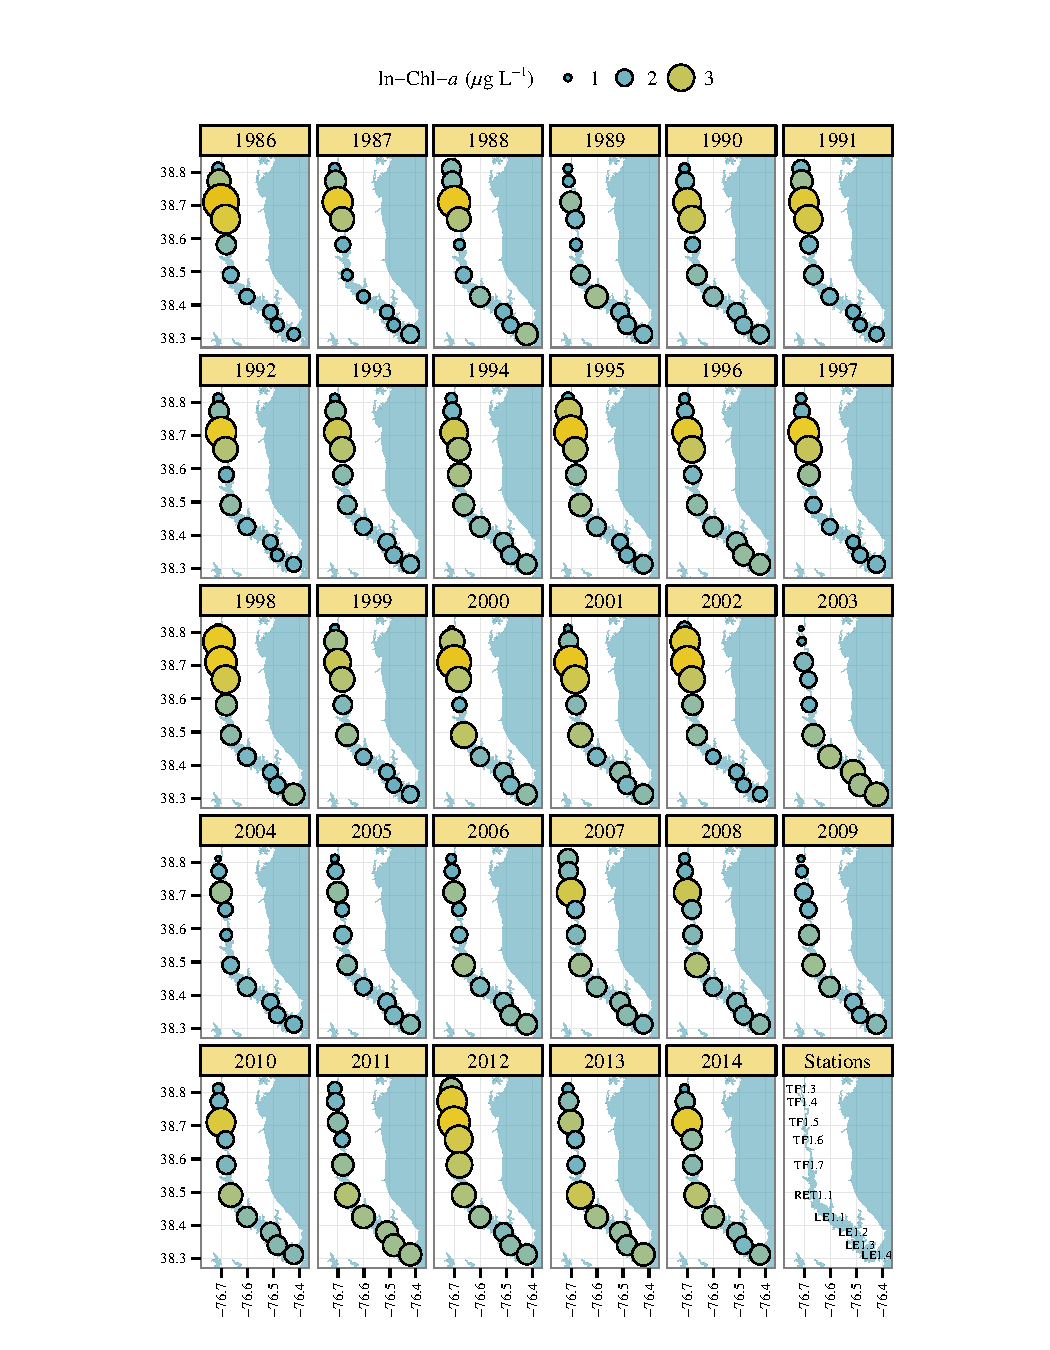
\includegraphics[width=\maxwidth]{figs/chlyr-1} 

}

\caption[Annual chlorophyll trends at each monitoring station in the Patuxent River Estuary]{Annual chlorophyll trends at each monitoring station in the Patuxent River Estuary.  Values are annual medians of ln-chlorophyll-a with size and color proportional between years.}\label{fig:chlyr}
\end{figure}



\begin{figure}[!ht]

{\centering 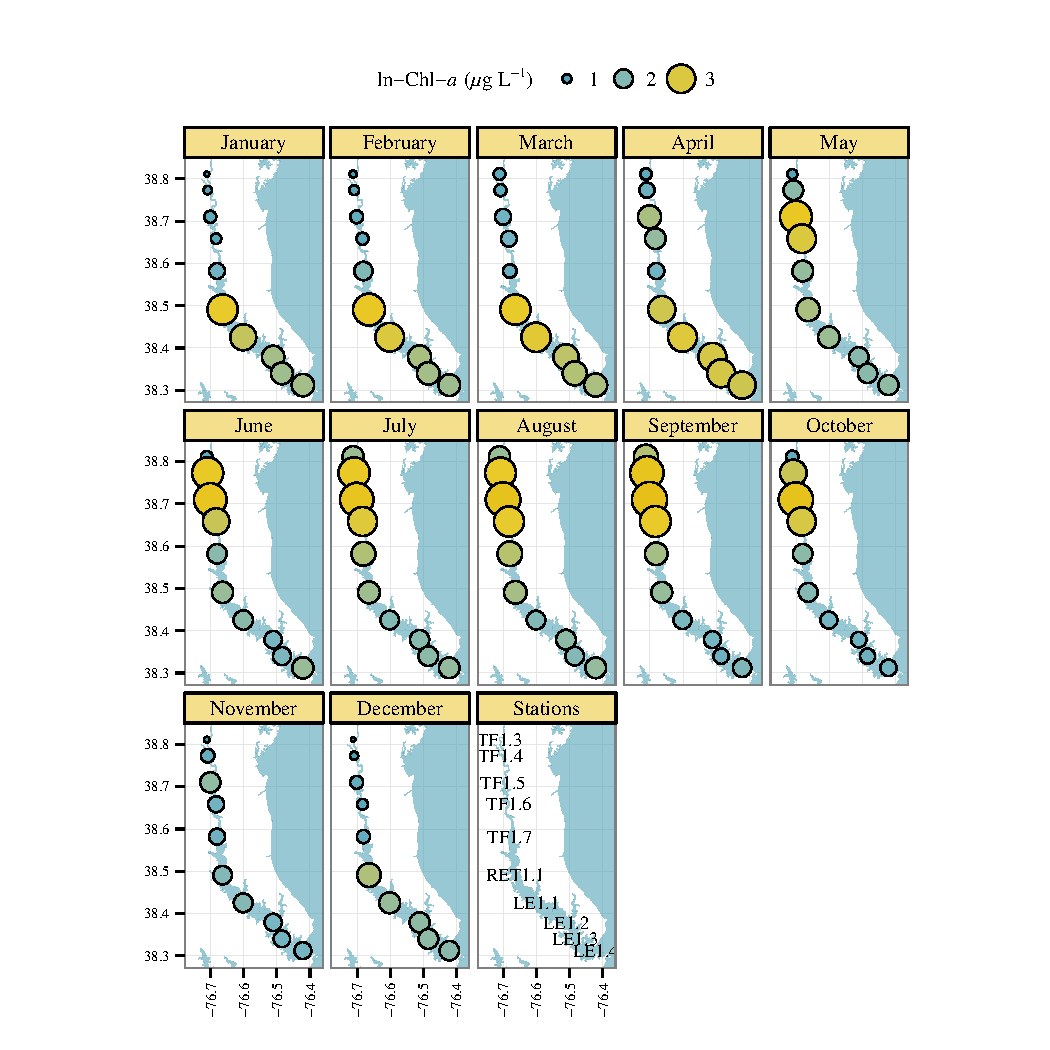
\includegraphics[width=\maxwidth]{figs/chlmo-1} 

}

\caption[Monthly chlorophyll trends at each monitoring station in the Patuxent River Estuary]{Monthly chlorophyll trends at each monitoring station in the Patuxent River Estuary.  Values are monthly medians of ln-chlorophyll-a with size and color proportional between months.}\label{fig:chlmo}
\end{figure}



% predicted trends for each mod - monthly time series of observed with predictions, RMSE in fig


% dynaplots for each mod (as in Fig. 8 Beck and Hagy 2015)

% scatterplot comparison of predictions between each mod (as in fig. 7 Moyer et al. 2012, incl ave diffs) - whole time series, different time periods (annual, seasonal groupings)

% histograms of errors for each mod, overlap with color transparencies - use period groupings as in previous fig

% examples of simulated datasets for eval of flow-normalization - daily, monthly, different flow effects

% results of flow-normalized data for simulations

\end{document}
